%%%%%%%%%%%%%%%%%%%%%%%%%%%%%%%%%%%%%%%%%%%%%%%%%%%%%%%%%%%%%%%%%%%%%
% LaTeX Template: Project Titlepage Modified (v 0.1) by rcx
%
% Original Source: http://www.howtotex.com
% Date: February 2014
% 
% This is a title page template which be used for articles & reports.
% 
% This is the modified version of the original Latex template from
% aforementioned website.
% 
%%%%%%%%%%%%%%%%%%%%%%%%%%%%%%%%%%%%%%%%%%%%%%%%%%%%%%%%%%%%%%%%%%%%%%

\documentclass[12pt]{report}
\usepackage[a4paper]{geometry}
\usepackage[myheadings]{fullpage}
\usepackage{fancyhdr}
\usepackage{lastpage}
\usepackage{graphicx, wrapfig, subcaption, setspace, booktabs}
\usepackage[T1]{fontenc}
\usepackage[font=small, labelfont=bf]{caption}
\usepackage{fourier}
\usepackage[protrusion=true, expansion=true]{microtype}
\usepackage[english]{babel}
\usepackage{sectsty}
\usepackage{url}
\usepackage{listings}
\usepackage{color}
\usepackage{xcolor}
\usepackage{etoolbox}
\usepackage{mdframed}
\newenvironment{theorem}%
  {\begin{mdframed}[backgroundcolor=lightgray]\begin{mdtheorem}}%
  {\end{mdtheorem}\end{mdframed}}

\AtBeginEnvironment{quote}{\singlespacing\small}

\newcommand{\HRule}[1]{\rule{\linewidth}{#1}}
\onehalfspacing
\setcounter{tocdepth}{5}
\setcounter{secnumdepth}{5}

\lstset { 
language=C++,
backgroundcolor=\color{black!10}, % set backgroundcolor
basicstyle=\footnotesize,% basic font setting
}
%-------------------------------------------------------------------------------
% HEADER & FOOTER
%-------------------------------------------------------------------------------
\pagestyle{fancy}
\fancyhf{}
\setlength\headheight{15pt}
\fancyhead[L]{FlatB}
\fancyhead[R]{Programming Manual}
\fancyfoot[R]{Page \thepage\ of \pageref{LastPage}}
%-------------------------------------------------------------------------------
% TITLE PAGE
%-------------------------------------------------------------------------------

\begin{document}

\title{ \normalsize \textsc{Programming Manual}
		\\ [2.0cm]
		\HRule{0.5pt} \\
		\LARGE \textbf{\uppercase{B Flat}}
		\HRule{2pt} \\ [0.5cm]
		\normalsize \today \vspace*{5\baselineskip}}

\date{}

\author{ Adarsh Sanjeev }

\maketitle
\tableofcontents
\newpage

%-------------------------------------------------------------------------------
% Section title formatting
\sectionfont{\scshape}
%-------------------------------------------------------------------------------

%-------------------------------------------------------------------------------
% BODY
%-------------------------------------------------------------------------------

\section*{Introduction}
\addcontentsline{toc}{section}{Introduction}
BFlat is a programming language

\section*{Syntax}
\addcontentsline{toc}{section}{Syntax}

\subsection*{Datatypes}
\addcontentsline{toc}{subsection}{Datatypes}

FlatB only has integers as valid datatypes for variables. However, strings are allowed as string literals for use in print statements.
The variables can be of array datatype also.

\subsection*{Statements}
\addcontentsline{toc}{subsection}{Statements}
Each statement in FlatB must end with a semicolon and be of one of the following types.

\subsubsection*{Assignment Statements}
\addcontentsline{toc}{subsubsection}{Assignment Statements}
Assignment statments must have a variable in the left hand side, and an expression in the right hand side.
\begin{lstlisting}
  x = 3;
  x = 2+4;
  x[2] = 4*4+2;
  x[y+2] = 5/3;
\end{lstlisting}

\subsubsection*{Print Statements}
\addcontentsline{toc}{subsubsection}{Print Statements}
Print statments can contain one or more comma separated values which can be strings or variables.
\begin{lstlisting}
print `Hello`, `World`;
print x[1], x[5];
\end{lstlisting}

\subsubsection*{Read Statements}
\addcontentsline{toc}{subsubsection}{Read Statements}
Read statments can contain one or more variables separated by commas.
\begin{lstlisting}
read x, y;
read x[5], y[2+2];
\end{lstlisting}

\subsubsection*{If Statement}
\addcontentsline{toc}{subsubsection}{If Statements}
\begin{lstlisting}
if ( x > 2) {
 //Statements
}
else {
 //Statements  
}
\end{lstlisting}

\subsubsection*{For loop}
\addcontentsline{toc}{subsubsection}{For Statements}
\begin{lstlisting}
for x=2, 5 { // Default step is +1
 //Statements
}

for x=2, 10, 2 {
 //Statements
}

for x=2, 9, 2 { // Won't terminate if condition is not met
 //Statements
}

\end{lstlisting}

\subsubsection*{While Loop Statement}
\addcontentsline{toc}{subsubsection}{While Loop}
\begin{lstlisting}
while ( x > 2) {
 //Statements
}
\end{lstlisting}

\subsubsection*{Goto Statement}
\addcontentsline{toc}{subsubsection}{Goto Statements}
\begin{lstlisting}
LABEL:
// Statements
goto LABEL;
goto LABEL if x > 2;
\end{lstlisting}

% \section*{Semantics}
% \addcontentsline{toc}{section}{Semantics}
\newpage
\section*{AST Design}
\addcontentsline{toc}{section}{AST Design}
\begin{figure}[h]
  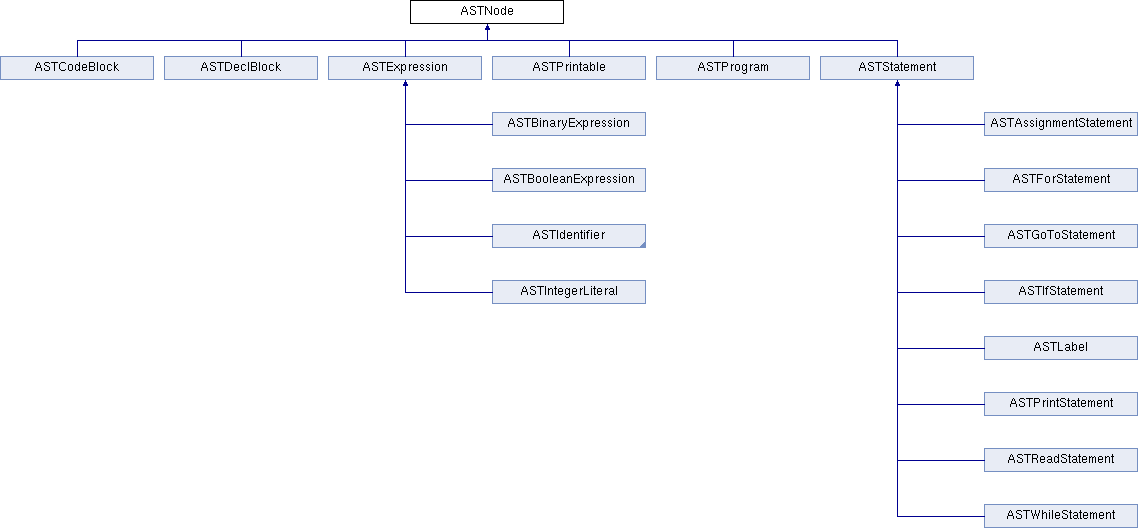
\includegraphics[width=\linewidth]{class_a_s_t_node.png}
  \caption{Inheritance Graph of ASTNode}
  \label{fig:figure1}
\end{figure}
\section*{Visitor Design Pattern}
\addcontentsline{toc}{section}{Visitor Design Pattern}
The visitor contains the visit function for all of the classes. The classes themselves contain the accept method for the visitor.
\begin{lstlisting}
virtual void* visit(ASTProgram *ast);
virtual void* visit(ASTDeclBlock *ast);
virtual void* visit(ASTCodeBlock *ast);
virtual void* visit(ASTIntegerLiteral *ast);
virtual void* visit(ASTIdentifier *ast);
virtual void* visit(ASTBinaryExpression *ast);
virtual void* visit(ASTBooleanExpression *ast);
virtual void* visit(ASTAssignmentStatement *ast);
virtual void* visit(ASTPrintStatement *ast);
virtual void* visit(ASTLabel *ast);
virtual void* visit(ASTReadStatement *ast);
virtual void* visit(ASTWhileStatement *ast);
virtual void* visit(ASTIfStatement *ast); 
virtual void* visit(ASTForStatement *ast);
virtual void* visit(ASTGoToStatement *ast);
\end{lstlisting}
\begin{figure}[h]
 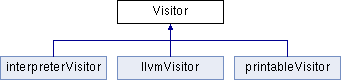
\includegraphics[width=\linewidth]{class_visitor.png}
 \caption{Inheritance Graph of Visitor}
 \label{fig:figure2}
\end{figure}
\section*{Design of Interpreter}
The interpreter implements a visitor. In the visitor class, it simply runs the code as C.
\section*{Design of LLVM Code Generator}
The code generator also implements a visitor. A llvm::Module is used to store the code, which is added by the various visit functions.
\begin{lstlisting}
void *visit (ASTProgram *ast)
void *visit (ASTCodeBlock *ast)
void *visit (ASTLabel *ast  
void *visit (ASTGoToStatement *ast)
void *visit (ASTDeclBlock *ast)
bool isDeclared (ASTIdentifier *ast)
void *visit (ASTAssignmentStatement *ast)
llvm::Value *convertToValue (string text)
void *visit (ASTReadStatement *ast)
void *visit (ASTPrintStatement *printStatement)
void *visit (ASTWhileStatement *ast)
void *visit (ASTIfStatement *ast)
void *visit (ASTBinaryExpression *ast)
void *visit (ASTBooleanExpression *ast)
void *visit (ASTIntegerLiteral *ast)
void *visit (ASTIdentifier *ast) 
void *visit (ASTForStatement *ast)
\end{lstlisting}
\section*{Performance Comparison}
\addcontentsline{toc}{section}{Performance Comparison}
\subsection*{Nested loops}
\addcontentsline{toc}{subsubsection}{Nested loops}
\begin{quote}
 Interpreter \\ 
                                                                                      \\ 
         64.959270      task-clock:u (msec)       \#    0.995 CPUs utilized           \\ 
                 0      context-switches:u        \#    0.000 K/sec                   \\ 
                 0      cpu-migrations:u          \#    0.000 K/sec                   \\ 
             1,644      page-faults:u             \#    0.025 M/sec                   \\ 
       165,019,321      cycles:u                  \#    2.540 GHz                     \\ 
       207,817,955      instructions:u            \#    1.26  insn per cycle          \\ 
        37,957,543      branches:u                \#  584.328 M/sec                   \\ 
           197,379      branch-misses:u           \#    0.52\% of all branches        \\ 
                                                                                      \\ 
       0.065293522 seconds time elapsed                                               \\ 
                                                                                      \\ 
LLI                                                                                     \\ 
                                                                                      \\ 
 Performance counter stats for 'lli ll-src/four nested loops.ll':                     \\ 
                                                                                      \\ 
         19.760535      task-clock:u (msec)       \#    0.987 CPUs utilized           \\ 
                 0      context-switches:u        \#    0.000 K/sec                   \\ 
                 0      cpu-migrations:u          \#    0.000 K/sec                   \\ 
             1,849      page-faults:u             \#    0.094 M/sec                   \\ 
        42,513,111      cycles:u                  \#    2.151 GHz                     \\ 
        64,944,168      instructions:u            \#    1.53  insn per cycle          \\ 
        11,852,773      branches:u                \#  599.820 M/sec                   \\ 
           240,822      branch-misses:u           \#    2.03\% of all branches        \\ 
                                                                                      \\ 
       0.020017150 seconds time elapsed                                               \\ 
                                                                                      \\ 
LLC                                                                                     \\ 
                                                                                      \\ 
 Performance counter stats for './ll-out/four nested loops':                          \\ 
                                                                                      \\ 
          3.762934      task-clock:u (msec)       \#    0.949 CPUs utilized           \\ 
                 0      context-switches:u        \#    0.000 K/sec                   \\ 
                 0      cpu-migrations:u          \#    0.000 K/sec                   \\ 
                96      page-faults:u             \#    0.026 M/sec                   \\ 
         9,120,774      cycles:u                  \#    2.424 GHz                     \\ 
        20,378,922      instructions:u            \#    2.23  insn per cycle          \\ 
         4,184,892      branches:u                \# 1112.135 M/sec                   \\ 
            20,664      branch-misses:u           \#    0.49\% of all branches        \\ 
                                                                                      \\ 
       0.003966169 seconds time elapsed                                               \\ 
\end{quote}

\subsection*{Bubblesort}
\addcontentsline{toc}{subsubsection}{Bubblesort}

\begin{quote}
 Interpreter \\ 
 Performance counter stats for './src/bci src/testcases/bubblesort.b':                \\ 
                                                                                      \\ 
       3781.533053      task-clock:u (msec)       \#    0.999 CPUs utilized           \\ 
                 0      context-switches:u        \#    0.000 K/sec                   \\ 
                 0      cpu-migrations:u          \#    0.000 K/sec                   \\ 
            11,321      page-faults:u             \#    0.003 M/sec                   \\ 
    10,167,104,493      cycles:u                  \#    2.689 GHz                     \\ 
    17,155,957,712      instructions:u            \#    1.69  insn per cycle          \\ 
     3,164,534,393      branches:u                \#  836.839 M/sec                   \\ 
         4,505,269      branch-misses:u           \#    0.14\% of all branches        \\ 
                                                                                      \\ 
       3.784120098 seconds time elapsed                                               \\ 
                                                                                      \\ 
LLI                                                                                     \\ 
                                                                                      \\ 
 Performance counter stats for 'lli ll-src/bubblesort.ll':                            \\ 
                                                                                      \\ 
         23.130742      task-clock:u (msec)       \#    0.989 CPUs utilized           \\ 
                 0      context-switches:u        \#    0.000 K/sec                   \\ 
                 0      cpu-migrations:u          \#    0.000 K/sec                   \\ 
             1,866      page-faults:u             \#    0.081 M/sec                   \\ 
        50,664,247      cycles:u                  \#    2.190 GHz                     \\ 
        64,035,872      instructions:u            \#    1.26  insn per cycle          \\ 
        11,100,635      branches:u                \#  479.908 M/sec                   \\ 
           292,971      branch-misses:u           \#    2.64\% of all branches        \\ 
                                                                                      \\ 
       0.023384569 seconds time elapsed                                               \\ 
                                                                                      \\ 
LLC                                                                                     \\ 
                                                                                      \\ 
 Performance counter stats for './ll-out/bubblesort':                                 \\ 
                                                                                      \\ 
          3.101557      task-clock:u (msec)       \#    0.940 CPUs utilized           \\ 
                 0      context-switches:u        \#    0.000 K/sec                   \\ 
                 0      cpu-migrations:u          \#    0.000 K/sec                   \\ 
               100      page-faults:u             \#    0.032 M/sec                   \\ 
         7,518,050      cycles:u                  \#    2.424 GHz                     \\ 
        14,464,612      instructions:u            \#    1.92  insn per cycle          \\ 
         2,367,470      branches:u                \#  763.317 M/sec                   \\ 
            20,241      branch-misses:u           \#    0.85\% of all branches        \\ 
                                                                                      \\
       0.003297922 seconds time elapsed                                               \\
\end{quote}

\subsection*{Fibonnacci}
\addcontentsline{toc}{subsubsection}{Fibonnacci}

\begin{quote}
 Interpreter \\ 
 Performance counter stats for './src/bci src/testcases/fibonnacci.b':             \\     
                                                                                   \\ 
         13.488520      task-clock:u (msec)       \#    0.984 CPUs utilized        \\   
                 0      context-switches:u        \#    0.000 K/sec                \\   
                 0      cpu-migrations:u          \#    0.000 K/sec                \\   
             1,448      page-faults:u             \#    0.107 M/sec                \\   
        28,853,790      cycles:u                  \#    2.139 GHz                  \\   
        41,284,026      instructions:u            \#    1.43  insn per cycle       \\   
         6,496,446      branches:u                \#  481.628 M/sec                \\   
           112,475      branch-misses:u           \#    1.73\% of all branches     \\    
                                                                                   \\ 
       0.013707329 seconds time elapsed                                            \\ 
                                                                                   \\ 
LLI                                                                                     \\ 
                                                                                   \\ 
 Performance counter stats for 'lli ll-src/fibonnacci.ll':                         \\ 
                                                                                   \\ 
         17.555911      task-clock:u (msec)       \#    0.981 CPUs utilized        \\   
                 0      context-switches:u        \#    0.000 K/sec                \\   
                 0      cpu-migrations:u          \#    0.000 K/sec                \\   
             1,845      page-faults:u             \#    0.105 M/sec                \\   
        35,972,370      cycles:u                  \#    2.049 GHz                  \\   
        48,363,807      instructions:u            \#    1.34  insn per cycle       \\   
         8,192,814      branches:u                \#  466.670 M/sec                \\   
           238,999      branch-misses:u           \#    2.92\% of all branches     \\    
                                                                                   \\ 
       0.017890038 seconds time elapsed                                            \\ 
                                                                                   \\ 
LLC                                                                                     \\ 
                                                                                   \\ 
 Performance counter stats for './ll-out/fibonnacci':                              \\ 
                                                                                   \\ 
          1.283848      task-clock:u (msec)       \#    0.857 CPUs utilized        \\   
                 0      context-switches:u        \#    0.000 K/sec                \\   
                 0      cpu-migrations:u          \#    0.000 K/sec                \\   
                94      page-faults:u             \#    0.073 M/sec                \\   
         2,615,905      cycles:u                  \#    2.038 GHz                  \\   
         4,302,589      instructions:u            \#    1.64  insn per cycle       \\   
           620,118      branches:u                \#  483.015 M/sec                \\   
            19,153      branch-misses:u           \#    3.09\% of all branches     \\    
                                                                                   \\ 
       0.001498751 seconds time elapsed                                            \\ 
\end{quote}

\subsection*{Matrix Multiplication}
\addcontentsline{toc}{subsubsection}{Matrix Multiplication}

\begin{quote}
 Interpreter \\ 

 Performance counter stats for './src/bci src/testcases/matrix multiplication.b':    \\ 
                                                                                     \\ 
         18.762214      task-clock:u (msec)       \#    0.984 CPUs utilized          \\ 
                 0      context-switches:u        \#    0.000 K/sec                  \\ 
                 0      cpu-migrations:u          \#    0.000 K/sec                  \\ 
             1,466      page-faults:u             \#    0.078 M/sec                  \\ 
        42,251,633      cycles:u                  \#    2.252 GHz                    \\ 
        66,893,002      instructions:u            \#    1.58  insn per cycle         \\ 
        11,357,038      branches:u                \#  605.314 M/sec                  \\ 
           123,818      branch-misses:u           \#    1.09\% of all branches       \\ 
                                                                                     \\ 
       0.019070266 seconds time elapsed                                              \\ 
                                                                                     \\ 
LLI                                                                                     \\ 
\\
 Performance counter stats for 'lli ll-src/matrix multiplication.ll':                \\ 
                                                                                     \\ 
         24.161403      task-clock:u (msec)       \#    0.990 CPUs utilized          \\ 
                 0      context-switches:u        \#    0.000 K/sec                  \\ 
                 0      cpu-migrations:u          \#    0.000 K/sec                  \\ 
             1,938      page-faults:u             \#    0.080 M/sec                  \\ 
        54,418,779      cycles:u                  \#    2.252 GHz                    \\ 
        73,403,594      instructions:u            \#    1.35  insn per cycle         \\ 
        13,353,191      branches:u                \#  552.666 M/sec                  \\ 
           442,419      branch-misses:u           \#    3.31\% of all branches       \\ 
                                                                                     \\ 
       0.024399177 seconds time elapsed                                              \\ 
                                                                                     \\ 
LLC                                                                                     \\ 
                                                                                     \\ 
 Performance counter stats for './ll-out/matrix multiplication':                     \\ 
                                                                                     \\ 
          1.255880      task-clock:u (msec)       \#    0.816 CPUs utilized          \\ 
                 0      context-switches:u        \#    0.000 K/sec                  \\ 
                 0      cpu-migrations:u          \#    0.000 K/sec                  \\ 
                99      page-faults:u             \#    0.079 M/sec                  \\ 
         2,586,835      cycles:u                  \#    2.060 GHz                    \\ 
         4,333,942      instructions:u            \#    1.68  insn per cycle         \\ 
           626,453      branches:u                \#  498.816 M/sec                  \\ 
            19,476      branch-misses:u           \#    3.11\% of all branches       \\ 
                                                                                     \\ 
       0.001539950 seconds time elapsed                                              \\ 
\end{quote}


% \begin{center}
% \begin{tabular}{ ll| l | c | r }
% \hline
% Four nested loops \\
% \hline
% &interpreter & lli & llc	\\
% &0m0.000s &	0m0.007s &	0m0.000s\\
% \hline
% Bubblesort \\
% \hline
% &interprer &  lli	 &   	llc		\\
% &0m0.017s &  0m0.007s &   0m0.000s\\
% \hline
% Fibonnacci\\
% \hline
% &interpreter &  lli	 &   	llc		\\
% &0m0.007s &  0m0.009s &   0m0.002s\\
% \hline
% Matrix Multiplication \\
% \hline
% &interpreter &  lli	 &   	llc	\\	
% &0m0.000s &  0m0.000s &   0m0.000s\\
% \hline
% \end{tabular}
% \end{center}

\end{document}

%-------------------------------------------------------------------------------
% SNIPPETS
%-------------------------------------------------------------------------------

%\begin{figure}[!ht]
%	\centering
%	\includegraphics[width=0.8\textwidth]{file_name}
%	\caption{}
%	\centering
%	\label{label:file_name}
%\end{figure}

%\begin{figure}[!ht]
%	\centering
%	\includegraphics[width=0.8\textwidth]{graph}
%	\caption{Blood pressure ranges and associated level of hypertension (American Heart Association, 2013).}
%	\centering
%	\label{label:graph}
%\end{figure}

%\begin{wrapfigure}{r}{0.30\textwidth}
%	\vspace{-40pt}
%	\begin{center}
%		\includegraphics[width=0.29\textwidth]{file_name}
%	\end{center}
%	\vspace{-20pt}
%	\caption{}
%	\label{label:file_name}
%\end{wrapfigure}

%\begin{wrapfigure}{r}{0.45\textwidth}
%	\begin{center}
%		\includegraphics[width=0.29\textwidth]{manometer}
%	\end{center}
%	\caption{Aneroid sphygmomanometer with stethoscope (Medicalexpo, 2012).}
%	\label{label:manometer}
%\end{wrapfigure}

%\begin{table}[!ht]\footnotesize
%	\centering
%	\begin{tabular}{cccccc}
%	\toprule
%	\multicolumn{2}{c} {Pearson's correlation test} & \multicolumn{4}{c} {Independent t-test} \\
%	\midrule	
%	\multicolumn{2}{c} {Gender} & \multicolumn{2}{c} {Activity level} & \multicolumn{2}{c} {Gender} \\
%	\midrule
%	Males & Females & 1st level & 6th level & Males & Females \\
%	\midrule
%	\multicolumn{2}{c} {BMI vs. SP} & \multicolumn{2}{c} {Systolic pressure} & \multicolumn{2}{c} {Systolic Pressure} \\
%	\multicolumn{2}{c} {BMI vs. DP} & \multicolumn{2}{c} {Diastolic pressure} & \multicolumn{2}{c} {Diastolic pressure} \\
%	\multicolumn{2}{c} {BMI vs. MAP} & \multicolumn{2}{c} {MAP} & \multicolumn{2}{c} {MAP} \\
%	\multicolumn{2}{c} {W:H ratio vs. SP} & \multicolumn{2}{c} {BMI} & \multicolumn{2}{c} {BMI} \\
%	\multicolumn{2}{c} {W:H ratio vs. DP} & \multicolumn{2}{c} {W:H ratio} & \multicolumn{2}{c} {W:H ratio} \\
%	\multicolumn{2}{c} {W:H ratio vs. MAP} & \multicolumn{2}{c} {\% Body fat} & \multicolumn{2}{c} {\% Body fat} \\
%	\multicolumn{2}{c} {} & \multicolumn{2}{c} {Height} & \multicolumn{2}{c} {Height} \\
%	\multicolumn{2}{c} {} & \multicolumn{2}{c} {Weight} & \multicolumn{2}{c} {Weight} \\
%	\multicolumn{2}{c} {} & \multicolumn{2}{c} {Heart rate} & \multicolumn{2}{c} {Heart rate} \\
%	\bottomrule
%	\end{tabular}
%	\caption{Parameters that were analysed and related statistical test performed for current study. BMI - body mass index; SP - systolic pressure; DP - diastolic pressure; MAP - mean arterial pressure; W:H ratio - waist to hip ratio.}
%	\label{label:tests}
%\end{table}
